\documentclass{standalone}

\usepackage{graphicx}
\usepackage{tikz}
\usetikzlibrary{angles,arrows.meta,decorations.pathmorphing,patterns,quotes,calc,decorations.pathreplacing,decorations.shapes,3d,plotmarks,positioning}

\usepackage[export]{adjustbox}
\usepackage[caption=false]{subfig}

\usepackage{pgfplots}
\pgfplotsset{compat=1.18}

\graphicspath{{../figures}}

%%%%%%%%%%% MATH %%%%%%%%%%%%
\usepackage{amsmath}
\usepackage{tensor}
\usepackage{upgreek}
\usepackage{sansmath}
\usepackage{xspace}
\usepackage{amsfonts}
\usepackage{array}

%% MATH MACROS
\newcommand{\ds}{\displaystyle}
\newcommand{\bs}[1]{\textsf{\textbf{#1}}}
\newcommand{\bm}[1]{\text{\boldmath{$#1$}}}

\begin{document}
	
	\begin{tikzpicture}
		\node[] (C) at (0, 0) %
			{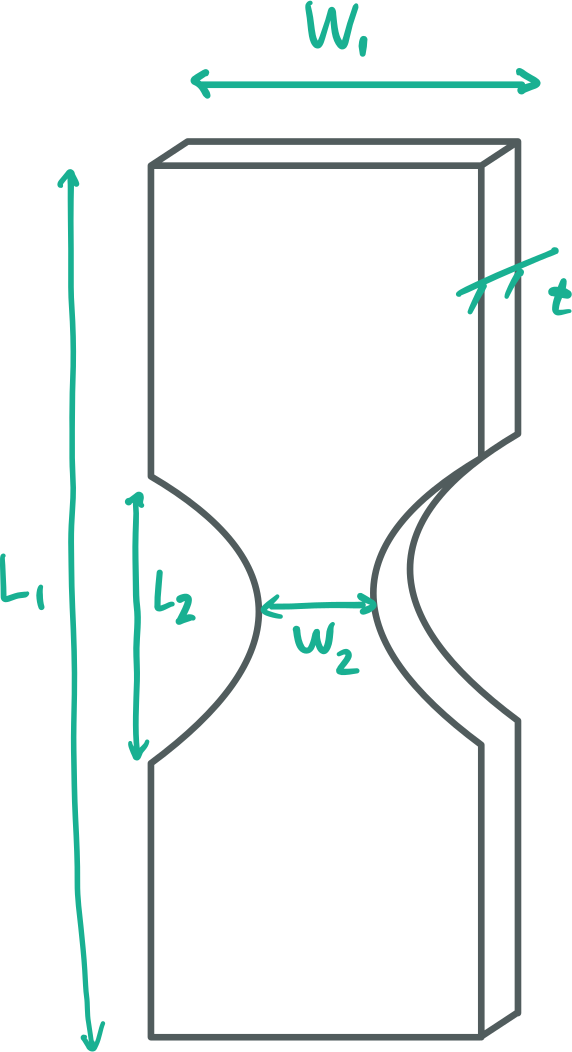
\includegraphics[height=6cm]{sample_sketch.png}};
		\node[anchor=north, text width=3.4cm] at (C.south) {(a) Sketch of sample.};
		
		\node[anchor=south west] (A) at ($(C.south east)+(5mm,0)$) %
			{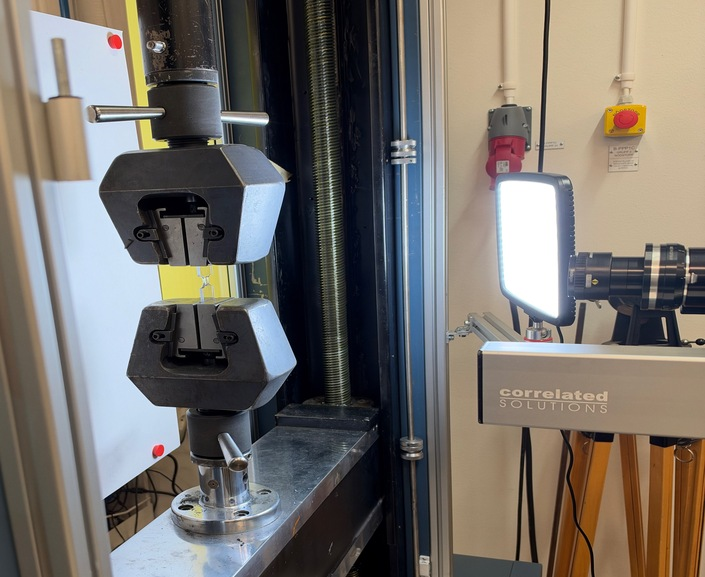
\includegraphics[height=6cm]{view_1_cropped.jpeg}};
		\node[anchor=north, text width=6cm] at (A.south) {(b) Sample mounted in machine.};
		
		\node[anchor=south west] (B) at (A.south east)%
			{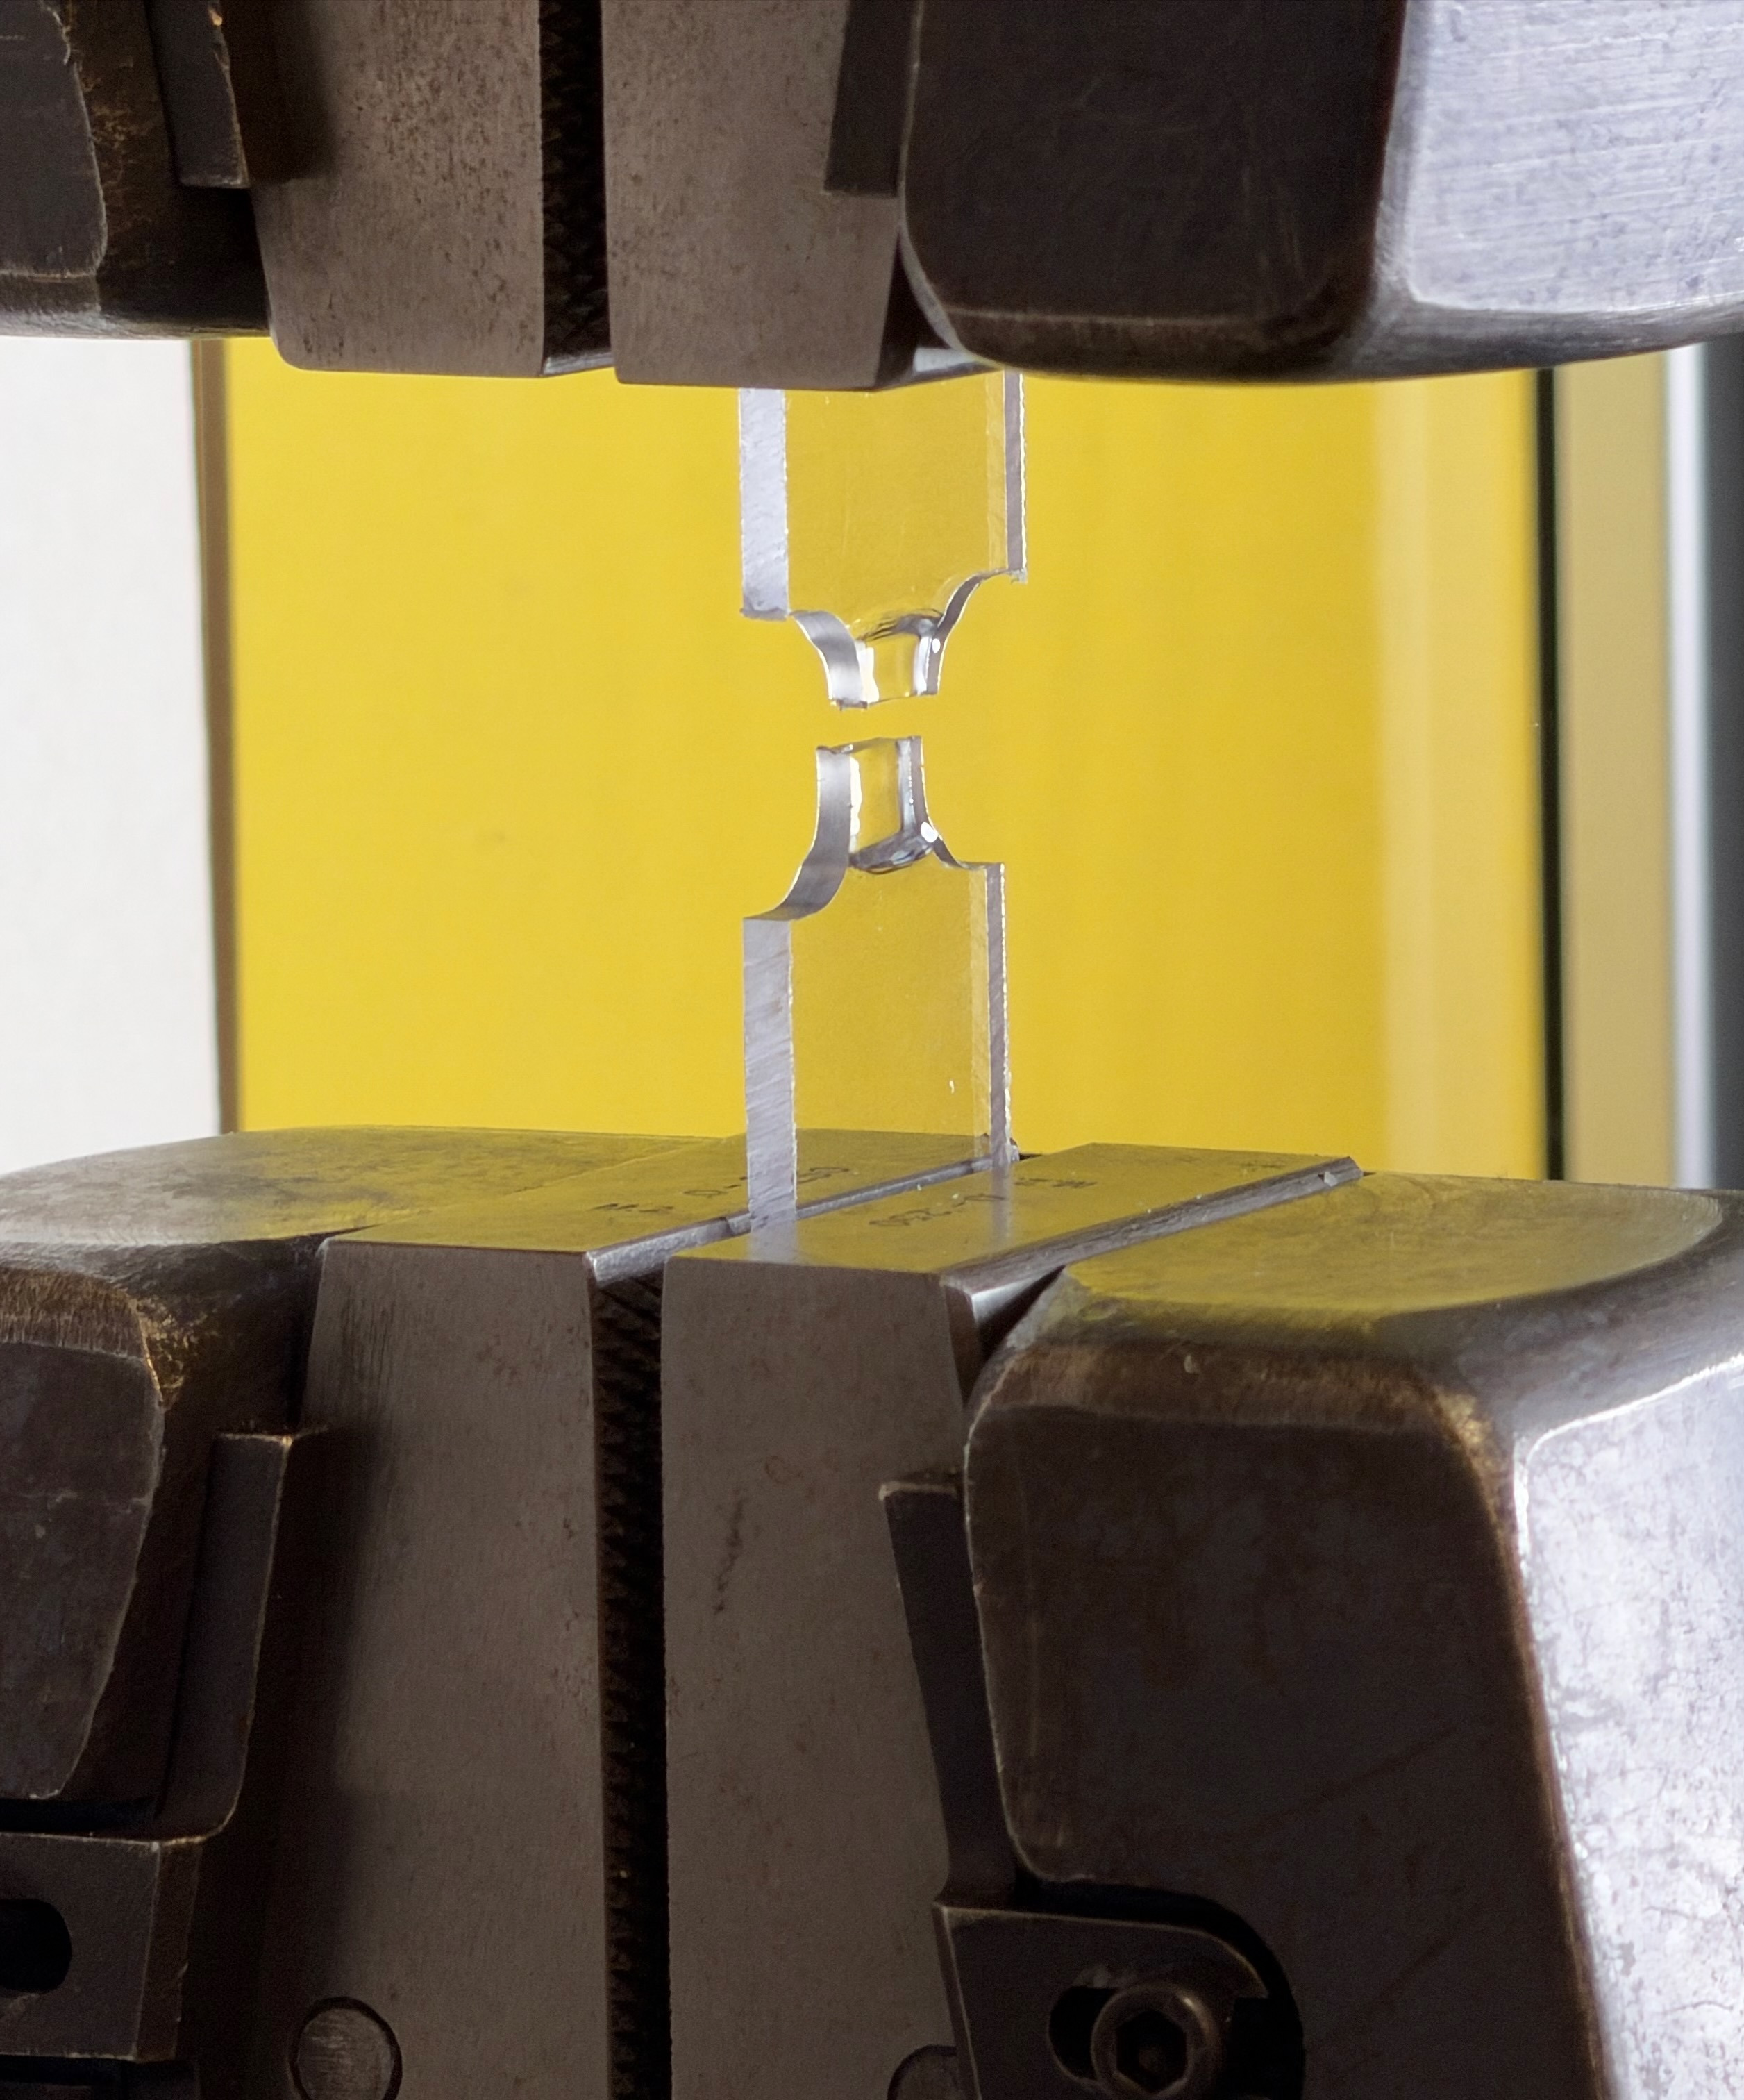
\includegraphics[height=6cm]{view_2_cropped.jpeg}};
		\node[anchor=north, text width=4cm] at (B.south) {(c) Zoomed in view of sample after tensile test.};
		
		\coordinate (O) at (5.8, 0);
		\coordinate (L1A) at ($(O) + ( 0.5,  1.5)$);
		\coordinate (L1B) at ($(O) + (-0.3,  1.2)$);
		\coordinate (L2B) at ($(O) + (-0.3, -0.5)$);
		\coordinate (L3A) at ($(O) + ( 0.5, -1.5)$);
		\coordinate (L3B) at ($(O) + (-1.2,  0.0)$);
		\draw[-Latex, color=blue] (L1A) -- (L1B);
		\draw[-Latex, color=blue] (L1A) -- (L2B) %
			node[at start,anchor=west, text width=2cm]{top/bottom holding grips};
			
			
		\draw[-Latex, color=green] (L3A) -- (L3B) %
			node[at start, anchor=west, text width=2cm]{sample};
		
	\end{tikzpicture}
	
\end{document}
